\section{Construction}
\subsection*{Cross-chain certificates}
For our construction, we use a primitive called Non-Interactive Proofs of
Proof-of-Work recently introduced in~\cite{nipopows}.
Non-Interactive Proofs of Proofs-of-Work are cryptographic protocols which
implement a \emph{prover} and a \emph{verifier}. The prover is a \emph{full
node} on the \emph{source blockchain}. The verifier does not have access to
that blockchain, but knows the source genesis block $\mathcal{G}$. The prover
wants to convince the verifier that an \emph{event} took place in the source
blockchain; for instance, a smart contract method was called with certain
parameters or that a payment was made into a particular address. Whether such an
event took place can easily be determined if one inspects the whole blockchain.
However, the prover wishes to convince the verifier by only sending a
\emph{succinct proof}, a short string which does not grow linearly  with the
size of the source blockchain, but, rather, \emph{polylogarithmically}. The
verifier must not be fooled by \emph{adversarial provers} who provide incorrect
proofs claiming that an event happened while in fact it didn't, or that it
didn't while in fact it did. These adversaries can also mine blocks, but the
honest parties are assumed to control the majority of computational power on
both the source and the target blockchain networks. To withstand such attacks,
the verifier accepts multiple proofs, at least one of which is assumed to have
been honestly generated (this assumption is necessary in standard blockchain
protocols in general~\cite{EPRINT:KKZG15,wust2016ethereum}). Comparing these
proofs against each other, the verifier extracts a reliable truth value
corresponding to the same value it would deduce if it were to be running a full
node on the blockchain itself. This property is the \emph{security} of NIPoPoWs
proven in~\cite{nipopows}.

The NIPoPoWs construction talks about \emph{predicates} evaluated on
blockchains, but we are interested in \emph{events}. We can translate from
events to predicates provable with NIPoPoWs. Specifically, given a genesis block
$\mathcal{G}$, a smart contract address \textsf{addr}, an event name
\textsf{Event}, and a series of event parameter values $(\textsf{param}_1,
\textsf{param}_2, \cdots, \textsf{param}_n)$, the predicate $e$ we wish to check
for truth is the following: \emph{Has the event named \textsf{Event} been fired
with parameters $(\textsf{param}_1, \textsf{param}_2, \cdots, \textsf{param}_n)$
by the smart contract residing in address \textsf{addr} on the blockchain with
genesis block $\mathcal{G}$ at least $k$ blocks ago?} This predicate
is (1) \emph{monotonic}, meaning that it starts with the value \textsf{false}
and, if it ever becomes \textsf{true}, it cannot ever change its value back as
the blockchain grows; (2) \emph{infix-sensitive}, meaning that its truth value
can be deduced by inspecting a polylogarithmically-bound number of blocks on the
blockchain (in our case one block, within which the event firing was confirmed);
and (3) \emph{stable}, meaning that, if one party deduces that its value is
\textsf{true}, then soon enough \emph{all} parties will deduce that its value is
\textsf{true}. This last property stems from the requirement that the event be
buried under $k$ blocks ensuring a blockchain reorganization up to $k$ blocks
ago cannot affect the predicate's value.

In order to determine whether an event took place, the NIPoPoW verifier function
\textsf{verify}$^{\mathcal{G},e}_{k,m}(\mathcal{P})$ accepts the event
description in the form of a blockchain predicate $e$, which we gave above, the
genesis block of the remote chain $\mathcal{G}$, as well as two security
parameters $k$ and $m$. These security parameters can be constants specified
when the sidechain system is created (concrete values for these are given
in~\cite{nipopows}). Subsequently, the NIPoPoW verifier accepts a set of
\emph{proofs} $\mathcal{P} = \{\pi_1, \pi_2, \cdots, \pi_n\}$ which it compares
and extracts a truth value for the predicate: Whether the event has taken place
in the remote blockchain or not. As long as at least one \emph{honestly
generated} proof $\pi_i$ is provided, the verifier's security ensures that the
output will correspond to whether the event actually occurred.

Our protocol works as follows. Whenever an event of interest occurs on the
source blockchain, the occurence of this event is observed by a source
blockchain honest node, who generates a NIPoPoW about it. The target blockchain
contains a smart contract with a method to accept and verify the veracity of
this proof. The node can then submit the proof to the smart contract by
broadcasting a transaction on the target blockchain. As soon as the proof is
validated by the smart contract, the target blockchain can elect to react to the
event as desired.

\noindent
\textbf{Adoption considerations. } Our construction has certain prerequisites
for both the source and the target blockchain before it can be adopted. In the
case of bidirectionally connected blockchains, both of them must satisfy the
source and the target blockchain prerequisites.

\begin{itemize}
  \item \textbf{The source blockchain} needs to support \emph{proofs} about it,
        which requires augmenting it with an \emph{interlink} vector, the
        details of which can be found in~\cite{popow}. This interlink vector
        can be added to a blockchain using a \emph{user-activated velvet
        fork}~\cite{nipopows,velvet}, which is performed without miner awareness
        and does not require a hard or soft fork. However, only events occuring
        \emph{after} the velvet fork can be proven. New blockchains can adopt
        this from genesis.
  \item \textbf{The target blockchain} needs to be able to run the above
        \textsf{verify} function. This function can be programmed in a
        Turing-complete language such as Solidity. If the source blockchain
        proof-of-work hash function is available as an opcode or pre-compiled
        smart contract within the target blockchain's VM the way, e.g.,
        Bitcoin's SHA256 hash function is available in Solidity, the
        implementation can be more gas-efficient.
\end{itemize}

\noindent
\textbf{Blockchain agnosticism. }
We underline the remarkable property that miners and full nodes of the target
blockchain do not need to be aware of the source blockchain at all. To them,
all information about the source blockchain is simply a string which is passed
as a parameter to a smart contract and can remain \emph{agnostic} to its
semantics as a proof. Additionally, miners and full nodes of the source
blockchain do not need to be aware of the target blockchain. Only the parties
interested in facilitating cross-chain events must be aware of both. Those
untrusted facilitators need to maintain an SPV node on the source blockchain
about which they generate their NIPoPoW. To broadcast their proof on the target
blockchain, they connect to target blockchain nodes and send the transaction
containing the NIPoPoW. Blockchain agnosticism allows users to initiate
cross-chain relationships between different blockchains \emph{dynamically}, as
long as the blockchains in question satisfy the above prerequisites.

\import{./}{algorithms/crosschain.tex}

\subsection*{Cross-chain events}

We give our \textsf{crosschain} construction in Algorithm~\ref{alg.crosschain}.
Initially, our communication will be unidirectional. In the next section, we
use two unidirectional channels to establish bidirectional communication. This
smart contract runs on the target blockchain and informs it about events that
took place in the source blockchain. It is parameterized by three parameters:
$k$ and $m$ are the underlying security parameters of the NIPoPoW protocol. The
value $z$ is a \emph{collateral} parameter, denominated in ether (or the native
currency of the blockchain in which the execution takes place) and is used to
incentivize honest participants to intervene in cases of false claims. The
contract utilizes the NIPoPoW \textsf{verify} function parameterized by the
event $e$, the remote genesis block $\mathcal{G}$ and the security parameters
$k$ and $m$. We do not give an explicit implementation of \textsf{verify}, as it
can be implemented in a straightforward manner by translating the pseudocode
listing of~\cite{nipopows}. For our purposes, it suffices to treat it as a black
box which, given a set of proofs, at least one of which is honestly generated,
returns the truth value of the respective predicate.

The contract allows detecting remote blockchain events and can be \emph{inherited}
by other contracts that wish to adopt its functionality. It works as follows.
First, the \textsf{initialize} method is called exactly once to configure the
contract, passing the \emph{hash} of the genesis block of the remote chain which
this contract will handle. This method is \textsf{internal} and can only be
called by the contract inheriting from it. Users of the contract can check  it
has been configured with the correct genesis block prior to using it. We note
that, while our algorithm does not reflect this to keep complexity low, it is
possible to have a contract interact with \emph{multiple} remote chains by
extending it to include multiple geneses.

\begin{figure}[H]
    \caption{A sequence diagram showing the actions of the untrusted SPV node
             when communicating with both blockchain networks and the lifecycle
             of an event submission}
    \centering
    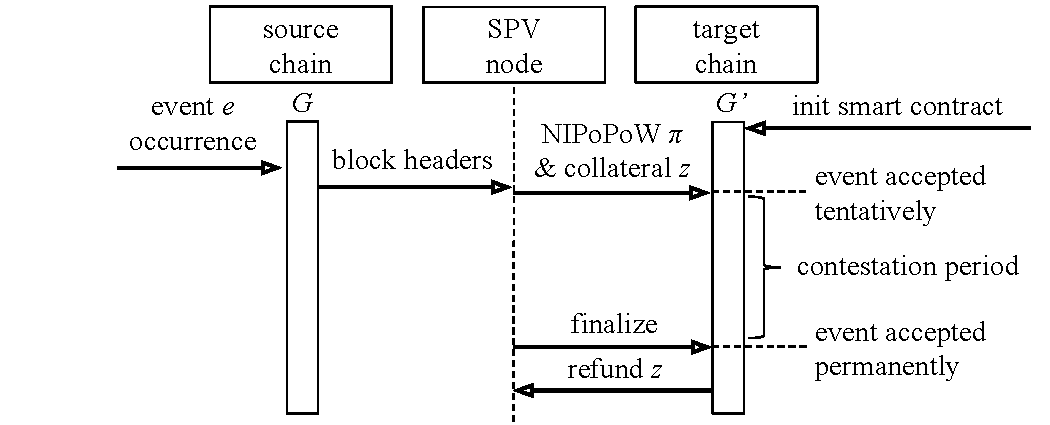
\includegraphics[width=0.9 \columnwidth,keepaspectratio]{figures/sequence-diagram.pdf}
    \label{fig.sequence}
\end{figure}

The lifecycle of an event submission is illustrated in
Figure~\ref{fig.sequence}. When an event has taken place in the source
blockchain, any source blockchain SPV node, the \emph{author}, can inform the
\textsf{crosschain} contract about this fact by generating a NIPoPoW $\pi$
claiming that the event took place based on their current view of the source
blockchain. This proof can then be submitted to the target blockchain by calling
the \textsf{submit-event-proof} function and passing it the proof $\pi$ and the
event predicate $e$. The submission is accompanied by a collateral payment $z$.
If the author is honest, this collateral will be returned to her later. The
\textsf{submit-event-proof} function runs the NIPoPoW \textsf{verify} algorithm
to check that the proof $\pi$ is well-formed and that it claims that the
predicate is \textsf{true}. It then stores the proof for later use. It also
stores the address of the \emph{author} and an \emph{expiration block number}.

Upon submission of a proof to the \textsf{submit-event-proof} function, the
event is \emph{tentatively accepted} for a \emph{contestation period} of $k$
blocks, during which any other party, the \emph{contester}, can provide a
counter-proof showing that the original proof was fraudulent. The contester can
call the \textsf{submit-contesting-proof} function passing it the contesting
proof $\pi^*$ and the event predicate $e$. The function runs the NIPoPoW
\textsf{verify} algorithm to compare the original proof
$\textsf{events}[e].\textsf{proof}$ against the contesting proof $\pi^*$. If the
verification algorithm concludes that the original proof was fraudulent, the
tentatively accepted event is abandoned and the collateral is paid to the
contester.

Otherwise, when the contestation period has expired without any valid
contestations, the author can call the \textsf{finalize-event} function. This
function changes the acceptance of the event from tentative to \emph{permanent}
by including it in the \textsf{finalized-events} set and returns the collateral
to the author. Finally, the \textsf{event-exists} function can be used by the
inheriting contract to check if an event has been permanently accepted. The
target blockchain state during this execution is shown in
Figure~\ref{fig.contestation}. The source blockchain's event included in the
black box, upon sufficient confirmation by $k_1$ blocks (not shown), is
transmitted to the target blockchain at the bottom. The target blockchain
includes the event \emph{tentatively} in block $1$ until a contestation period
of $k_2$ has passed; the event is included \emph{permanently} in block $2$;
subsequently, permanent inclusion needs to be confirmed with $k_2$ further
blocks.

\begin{figure}
    \caption{The target blockchain state during event submission}
    \centering
    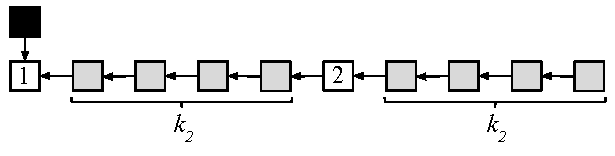
\includegraphics[width=0.6 \columnwidth,keepaspectratio]{figures/contestation.pdf}
    \label{fig.contestation}
\end{figure}

\subsection*{Two-way pegged sidechains}
Having created the generic crosschain contract, we now build two-way pegged
sidechains on top. For concreteness, we use the example of transferring ether
(ETH), the native currency of the Ethereum blockchain, to the Ethereum Classic
blockchain, and back. We note that this example is arbitrary and for
illustration. Our construction can be used between any work-based blockchains
satisfying the prerequisites detailed above.

When ether is moved to the Ethereum Classic blockchain, it will be represented
as an ERC20 token\footnote{The ERC20 standard~\cite{erc20} defines an interface
implementable by smart contracts that enables holding and transferring custom
fungible tokens such as ICO tokens.} within Ethereum Classic. Let this custom
token be called ETH20. The asset retains its nature as it moves from one
blockchain to another if it is always possible to move ETH into ETH20 and back
at a one-to-one rate. The economic reason is that the price of ETH and ETH20 on
the market will necessarily be the same. If the price of ETH were to ever be
significantly above the price of ETH20 in the market, then a rational
participant would exchange their ETH20 for ETH using sidechains and sell their
ETH on the market instead, and vice versa. There can be a small discrepancy in
the two prices which stems from two different factors: First, the fees needed
for a cross-chain transfer; and second, the temporary market fluctuations that
can occur during the limited time needed to perform the cross chain transfer
($k_1 + 2k_2$). If we assume the price fluctuation (of ETH20 denominated in ETH)
per unit of time is bounded, then the market price difference between ETH and
ETH20 at any moment in time can be bounded by the sum of these two factors.

The sidechain smart contracts are presented in Algorithm~\ref{alg.sidechain}.
These smart contracts both extend the \textsf{crosschain} smart contract of
Algorithm~\ref{alg.crosschain}. Furthermore, \textsf{sidechain}$_2$ also
inherits basic \textsf{ERC20} functionality which allows token owners to
transfer the token~\cite{openzeppelin-erc20}. The \textsf{sidechain}$_1$
contract will be instantiated on Ethereum, while the \textsf{sidechain}$_2$
contract will be instantiated on Ethereum Classic. Suppose the genesis block
hash of Ethereum is $\mathcal{G}_1$ and of Ethereum Classic is $\mathcal{G}_2$.
We will use the genesis block hash of each blockchain as its unique identifier.

The two smart contracts both contain an \textsf{initialize} method which accepts
the hash of the remote blockchain as well as the address of the remote smart
contract it will interface with. Note that, while the two genesis hashes can be
hard-coded into the respective smart contract code itself, the remote contract
address cannot be built-in as a constant into the smart contract, but must be
later specified by calling the \textsf{initialize} function. The reason is that,
if \textsf{sidechain}$_1$ were to be created on $\mathcal{G}_1$, it would
require the address of \textsf{sidechain}$_2$ to exist prior to its creation,
and vice versa in a circular dependency. Therefore, the two contracts must first
be created on their respective blockchain to obtain addresses, and then their
\textsf{initialize} methods can be called to inform each contract about the
address of the other. Specifically, first the contract \textsf{sidechain}$_1$ is
created on $\mathcal{G}_1$ to obtain its instance address which we also
denote \textsf{sidechain}$_1$. Then the second contract, \textsf{sidechain}$_2$,
is created on $\mathcal{G}_2$ to obtain its address \textsf{sidechain}$_2$.
Subsequently, the \textsf{initialize} function of \textsf{sidechain}$_1$ is
called, passing it $\mathcal{G}_2$ and the address \textsf{sidechain}$_2$.
Finally, \textsf{initialize} is called on \textsf{sidechain}$_2$, passing it
$\mathcal{G}_1$ and the address \textsf{sidechain}$_1$. These initialization
parameters are stored by the respective smart contracts for future use. As the
\textsf{crosschain} contract requires, the \textsf{initialize} method can only
be called once. Any user wishing to utilize this sidechain is expected to
validate that the contracts have been set up correctly and that
\textsf{initialize} has been called with the appropriate parameters.

\textsf{sidechain}$_1$ contains a \textsf{deposit} function
which is \emph{payable} in the native asset of Ethereum, ETH. When a user pays
ETH into the \textsf{deposit} function, the funds are held by the smart contract
and can later be used to pay parties who wish to \emph{withdraw}, an operation
performed by calling the \textsf{withdraw} function. \textsf{sidechain}$_2$
contains similar \textsf{deposit} and \textsf{withdraw} functions which,
however, do not pay in the native currency of Ethereum Classic, but instead
maintain a \textsf{balance} mapping akin to a typical ERC20 implementation. The
balance is updated when a user deposits or withdraws.

Moving funds from the Ethereum blockchain into the Ethereum Classic blockchain
works as follows. First, the user pays with ETH to call the \textsf{deposit}
function of \textsf{sidechain}$_1$ which resides on $\mathcal{G}_1$, passing the
\textsf{target} parameter which indicates their address in the Ethereum Classic
blockchain that they wish to receive the money into. This call emits an event,
\textsf{Deposited}$_1$ which contains the necessary data: the \textsf{target},
the \textsf{amount} paid, as well as a nonce \textsf{ctr} to allow for future
payments of the same amount to the same target. When the event has been emitted
and buried under $k_1$ blocks within the Ethereum blockchain, the user produces
an Ethereum NIPoPoW $\pi_1$ about the predicate $e_1$ which claims that the
event \textsf{Deposited}$_1$ has been emitted in blockchain $\mathcal{G}_1$ with
the particular parameters by the contract residing at address
\textsf{sidechain}$_1$.
% We
% will slightly abuse notation for event predicates and let $e_1$ be specified by
% the tuple containing the contract address, event name and parameters
% $(\textsf{sidechain}_1, \textsf{Deposited}_1, (\textsf{amount}, \textsf{target},
% \textsf{ctr}))$, noting that there is an obvious correspondence between the two.

\import{./}{algorithms/sidechain.tex}

Subsequently, the user calls the \textsf{submit-event-proof} function of
\textsf{sidechain}$_2$ (which is inherited from the \textsf{crosschain}
contract), passing the NIPoPoW $\pi_1$ and the event predicate $e_1$ and paying
collateral $z$, which registers $e_1$ on \textsf{sidechain}$_2$ as tentative.
Because the user is honest, no adversary can produce a $\pi^*_1$
which disproves their claim during the dispute period, and therefore the user
waits for $k_2$ blocks for the contestation period to expire without any
successful contestations. She then calls the \textsf{finalize-event} function
for $e_1$ and receives back the collateral $z$, marking the event permanent.
Finally, she calls the function \textsf{withdraw} of \textsf{sidechain}$_2$,
passing it the same parameters that $e_1$ was issued with. The \textsf{withdraw}
function checks that $e_1$ exists using the \textsf{event-exists} method, which
will return \textsf{true}. The user is then credited with \textsf{amount} in
their ETH20 balance stored in $\textsf{balances}[\textsf{target}]$. This
increment in balance creates brand new ETH20 tokens. The \textsf{withdraw}
function also stores the signature of the event parameters that have been spent
to avoid replay attacks, which is not shown here for algorithm brevity.

The user can then transfer their ETH20 tokens by utilizing the functionality
inherited from the \textsf{ERC20} contract.  When some (not necessarily the
same) user is ready to move some (not necessarily the same) amount of ETH20 from
the Ethereum Classic blockchain back into ETH on the Ethereum blockchain, they
follow the reverse procedure: They call the \textsf{withdraw}
function of \textsf{sidechain}$_2$ which ensures their ERC20 balance is
sufficient, deduces the requested amount, and fires an event $e_2$ as before. At
this point, these particular ETH20 tokens are destroyed by the balance
deduction. Once $e_2$ is confirmed in $\mathcal{G}_2$, the user produces the
NIPoPoW $\pi_2$ about $e_2$ which claims a payment was made within
$\mathcal{G}_2$. That proof is then submitted to \textsf{sidechain}$_1$ by
calling the \textsf{submit-event-proof} and \textsf{finalize-event} functions as
before. Last, the user calls the \textsf{withdraw} function of
\textsf{sidechain}$_1$, which uses the \textsf{event-exists} function which will
return \textsf{true}, finally paying back the user the respective amount of ETH.
Because the only way to create ETH20 tokens in \textsf{sidechain}$_2$ is by
depositing ETH into \textsf{sidechain}$_1$, there will always exist a sufficient
balance of ETH owned by the \textsf{sidechains}$_1$ smart contract to pay for
any requested withdrawals.

Suppose now that an adversarial user makes a false claim that an event $e$ took
place in $\mathcal{G}_1$ and posts a relevant NIPoPoW $\pi$ in $\mathcal{G}_2$.
If an honest party is monitoring the chain $\mathcal{G}_2$ for the appearance of
NIPoPoWs and the chain $\mathcal{G}_1$ for the firing of events, the fraudulence
of $\pi$ will be immediately obvious to them. They can subsequently generate a
contesting NIPoPoW $\pi^*$ providing a counter-claim that $e$ did not occur. The
honest party will broadcast this transaction at the beginning of the
contestation period. Due to the \emph{liveness} property of $\mathcal{G}_2$, the
honest party will manage to include this transaction into $\mathcal{G}_2$ within
one of the blocks before the end of the contestation period. The collateral $z$
must be sufficient to incentivize an honest party to monitor $\mathcal{G}_1$ and
$\mathcal{G}_2$ simultaneously, pay for transaction fees and ensure the time
needed to generate a NIPoPoW $\pi^*$ is small as compared to block generation
time. The argument for $\mathcal{G}_2$ is analogous. We make this security
argument formal in the appendix.
